\documentclass[11pt,oneside]{article}
\usepackage[a4paper,margin=25mm,headheight=15pt]{geometry}
\usepackage[T1]{fontenc}
\usepackage[utf8]{inputenc}
\IfFileExists{libertinus.sty}{\usepackage{libertinus}}{\usepackage{lmodern}}
\usepackage{microtype}
\usepackage{amsmath,amssymb,amsthm,mathtools,mathrsfs,bm}
\usepackage{booktabs,longtable,array,tabularx}
\usepackage{graphicx}
\usepackage{xcolor}
\usepackage{enumitem}
\usepackage{fancyhdr}
\usepackage{titlesec}
\usepackage{listings}
\usepackage{tcolorbox}
\tcbuselibrary{breakable,skins}
\usepackage{xurl}
\usepackage{hyperref}
\usepackage[nameinlink,noabbrev]{cleveref}

\definecolor{deepblue}{RGB}{29,67,113}
\definecolor{teal}{RGB}{25,105,101}
\definecolor{burgundy}{RGB}{125,48,63}
\definecolor{gold}{RGB}{157,111,27}
\definecolor{softblue}{RGB}{240,245,250}
\definecolor{softteal}{RGB}{238,248,247}
\definecolor{softgold}{RGB}{253,248,235}
\definecolor{softred}{RGB}{252,241,243}
\definecolor{rulegray}{RGB}{194,201,208}
\definecolor{codegray}{RGB}{247,248,250}

\hypersetup{
  colorlinks=true,
  linkcolor=deepblue,
  citecolor=teal,
  urlcolor=deepblue,
  pdftitle={Closed All-Orders Endpoint Asymptotics for the Inverse Fabius Function},
  pdfsubject={Diagonal Lagrange-Buermann reversion, periodic coefficient laws, and inverse derivatives},
  pdfkeywords={Fabius function, inverse Fabius function, Rvachev up-function, Lambert W, Lagrange inversion, Bell polynomials, Thue-Morse, q-binomial, sinc product}
}

\pagestyle{fancy}
\fancyhf{}
\fancyhead[L]{\small Inverse Fabius endpoint asymptotics}
\fancyhead[R]{\small All-orders coefficient calculus}
\fancyfoot[C]{\thepage}
\renewcommand{\headrulewidth}{0.4pt}
\titleformat{\section}{\Large\bfseries}{\thesection}{0.7em}{}
\titleformat{\subsection}{\large\bfseries}{\thesubsection}{0.7em}{}
\titleformat{\subsubsection}{\normalsize\bfseries}{\thesubsubsection}{0.7em}{}
\setcounter{secnumdepth}{3}
\setcounter{tocdepth}{2}
\setlist[itemize]{leftmargin=2em,itemsep=0.25em,topsep=0.4em}
\setlist[enumerate]{leftmargin=2.3em,itemsep=0.25em,topsep=0.4em}
\setlength{\emergencystretch}{3em}
\allowdisplaybreaks[2]
\numberwithin{equation}{section}

\newtheorem{theorem}{Theorem}[section]
\newtheorem{proposition}[theorem]{Proposition}
\newtheorem{lemma}[theorem]{Lemma}
\newtheorem{corollary}[theorem]{Corollary}
\newtheorem{conjecture}[theorem]{Conjecture}
\theoremstyle{definition}
\newtheorem{definition}[theorem]{Definition}
\newtheorem{algorithm}[theorem]{Algorithm}
\newtheorem{example}[theorem]{Example}
\theoremstyle{remark}
\newtheorem{remark}[theorem]{Remark}
\newtheorem{warning}[theorem]{Warning}

\newtcolorbox{resultbox}[1][]{
  enhanced,breakable,colback=softteal,colframe=teal,
  boxrule=0.65pt,arc=2pt,left=7pt,right=7pt,top=6pt,bottom=6pt,
  title={#1},fonttitle=\bfseries}
\newtcolorbox{statusbox}[1][]{
  enhanced,breakable,colback=softblue,colframe=deepblue,
  boxrule=0.65pt,arc=2pt,left=7pt,right=7pt,top=6pt,bottom=6pt,
  title={#1},fonttitle=\bfseries}
\newtcolorbox{cautionbox}[1][]{
  enhanced,breakable,colback=softgold,colframe=gold,
  boxrule=0.65pt,arc=2pt,left=7pt,right=7pt,top=6pt,bottom=6pt,
  title={#1},fonttitle=\bfseries}
\newtcolorbox{frontierbox}[1][]{
  enhanced,breakable,colback=softred,colframe=burgundy,
  boxrule=0.65pt,arc=2pt,left=7pt,right=7pt,top=6pt,bottom=6pt,
  title={#1},fonttitle=\bfseries}

\lstdefinestyle{reportcode}{
  basicstyle=\ttfamily\small,
  backgroundcolor=\color{codegray},
  frame=single,
  rulecolor=\color{rulegray},
  columns=fullflexible,
  keepspaces=true,
  showstringspaces=false,
  breaklines=true,
  xleftmargin=0.5em,
  xrightmargin=0.5em,
  aboveskip=0.8em,
  belowskip=0.8em,
  keywordstyle=\color{deepblue}\bfseries,
  commentstyle=\color{teal}
}

\newcommand{\R}{\mathbb R}
\newcommand{\C}{\mathbb C}
\newcommand{\Z}{\mathbb Z}
\newcommand{\e}{\mathrm e}
\newcommand{\ii}{\mathrm i}
\newcommand{\dd}{\,\mathrm d}
\newcommand{\eps}{\varepsilon}
\newcommand{\cO}{\mathcal O}
\newcommand{\smallo}{o}
\newcommand{\Bell}{\mathcal B}
\newcommand{\Cl}{\operatorname{Cl}}
\newcommand{\ind}{\mathbf 1}
\newcommand{\coeff}[2]{[z^{#1}]\,#2}
\newcommand{\wcoeff}[2]{[w^{#1}]\,#2}
\newcommand{\diagcoeff}[3]{[z^{#1}w^{#2}]\,#3}
\newcommand{\Psihat}{\widehat\Psi}
\newcommand{\Gzero}{G_0}
\newcommand{\Csharp}{C_{\sharp}}
\newcommand{\statusrepo}{\textsc{Repository input}}
\newcommand{\statusnew}{\textsc{Derived here}}
\newcommand{\statusconj}{\textsc{Conjectural}}

\begin{document}
\hypersetup{pageanchor=false}

\begin{titlepage}
\centering
\vspace*{1.5cm}
{\Huge\bfseries Closed All-Orders Endpoint Asymptotics\\[0.25em]
for the Inverse Fabius Function\par}
\vspace{0.8cm}
{\Large Diagonal Lagrange--Bürmann reversion, periodic top-jet laws,\\
phase-locked quantiles, and inverse-derivative hierarchies\par}
\vspace{1.2cm}
{\large Research report based on the complete LaTeX corpus under\\
\texttt{Analysis/FabiusFunction/docs}\par}
\vfill
\begin{tcolorbox}[enhanced,colback=softteal,colframe=teal,width=0.92\textwidth,boxrule=0.8pt,arc=3pt]
\textbf{Principal contribution.}
Starting from the repository's exact-phase forward expansion and its existing recursive inverse engine, this report gives a nonrecursive diagonal Lagrange--Bürmann formula for every inverse coefficient.  It proves coefficient-degree and highest-periodic-derivative laws, writes the third inverse correction explicitly, develops an all-order derivative calculus, and verifies the first three corrections on exact dyadic quantiles.
\end{tcolorbox}
\vfill
{\large 28 August 2026\par}
\end{titlepage}
\hypersetup{pageanchor=true}

\pagenumbering{roman}
\begin{abstract}
Let $F$ be the Fabius distribution function and $G=F^{-1}$.  The repository establishes an arbitrary-order small-$x$ expansion of $\log F(x)$ in the exact lower-Lambert phase $\lambda=-W_{-1}(-x\log2)/\log2$, with a one-periodic Gamma--zeta fluctuation $\Psi$ and periodic saddle coefficients $A_j$.  A recent inverse-focused draft in the same corpus already derives the first two endpoint corrections for $G$, their nontrivial phase dependence, and a triangular all-orders recursion.

This report closes the remaining coefficient-formula gap.  With
\[
 T=\log(1/y),\qquad \rho=\sqrt{\frac{2T}{\log2}},\qquad
 \ell=\log\rho,\qquad \theta=\rho+\frac1{\log2}+\frac12,
\]
we prove, for every fixed $N$, the two-scale expansion
\[
 G(y)=\Gzero(y)\left(1+\sum_{n=1}^{N}\frac{g_n(\ell,\theta)}{\rho^n}
 +\cO_N\!\left(\frac{(1+\ell)^{N+1}}{\rho^{N+1}}\right)\right),
\qquad
 \Gzero(y)=\frac{\sqrt T}{\e\sqrt{\log2}}\e^{-\sqrt{2T\log2}}.
\]
The coefficients are polynomials in $\ell$ with analytic one-periodic coefficients.  A catalytic-variable application of Lagrange--Bürmann inversion gives a finite coefficient extraction formula for every phase coefficient $d_n$, every logarithmic coefficient $h_n$, and every multiplicative coefficient $g_n$.  This is a direct formula rather than a step-by-step reversion.

Several structural consequences follow.  The universal highest logarithm is
$[\ell^n]g_n=1/(2^n n!)$.  The coefficient of the newest periodic derivative is
\[
 [\Psi^{(2n-2)}]h_n=[\Psi^{(2n-2)}]g_n
 =\frac{(-1)^n}{2^{n-1}(n-1)!(\log2)^{2n-2}}.
\]
We also obtain an explicit third correction, phase-locked all-orders subsequences, Gamma--zeta convolution formulas for Fourier modes, an all-order recurrence for the quantile elasticity, and for each fixed $m\ge1$ the two-term derivative law
\[
 G^{(m)}(y)=(-1)^{m-1}(m-1)!\frac{G(y)}{y^m\rho}
 \left[1+\frac{(\Psi'(\theta)-1)/\log2-H_{m-1}}{\rho}
 +\cO_m\!\left(\frac{1+\ell}{\rho^2}\right)\right].
\]
Exact tests at $y_n=F(2^{-n})$ show that the new third correction lowers the relative error to $7.40\times10^{-5}$ at $n=20$, $6.05\times10^{-7}$ at $n=80$, and $4.92\times10^{-8}$ at $n=160$.
\end{abstract}

\tableofcontents
\clearpage
\pagenumbering{arabic}

\section{Scope, corpus audit, and contribution boundary}
\label{sec:scope}

\subsection{The source corpus}
The requested source tree is unusually broad.  It contains the primary Fabius--Rvachev exposition, a canonical non-formalized frontier volume, historical versions, a Lean crosswalk, q-series and Thue--Morse studies, papers transcribed into LaTeX, and a rapidly growing set of frontier reports.  The inverse-and-sampling report records a recursive audit of 57 LaTeX sources in the pre-consolidation tree.  On 28 August 2026 the draft manifest reorganized later arrivals into thematic consolidations: Fourier decay, Thue--Morse, exponent and q-series, spectra and arithmetic, integration and transforms, inverse and sampling, representations, and collected frontiers.

For nonduplication, the audit was claim-oriented rather than merely bibliographic.  Every identified source was searched for the endpoint variables, inverse notation, Lambert phase, $\Psi$, $A_j$, Bell reversion, Lagrange inversion, derivative asymptotics, and coefficient-structure statements.  The endpoint and inverse sources were read line by line; unrelated transform, representation, interpolation, and Fourier-decay sources were read through their abstracts, contents, theorem statements, conclusion, and cross-references.  Historical variants were retained in the comparison because some contain formulas absent from the living exposition.

\begin{table}[ht]
\centering
\small
\begin{tabularx}{\textwidth}{@{}p{0.23\textwidth}X p{0.20\textwidth}@{}}
\toprule
Source family & Material relevant to this report & Audit role \\
\midrule
Primary exposition & Exact lower-Lambert phase; $\Csharp$, $\Psi$; $A_1,A_2$; arbitrary-order forward expansion & Analytic input \\
Canonical frontier volume & Closed saddle jets, Bell recurrences, top-jet law for $A_j$, explicit higher corrections & Coefficient input \\
Inverse and Sampling Frontiers & First two inverse corrections, cluster interval, two-term elasticity, triangular all-order engine & Immediate prior art \\
Archived small-argument studies & Earlier leading equivalents and derivative estimates & Historical boundary \\
q-series and Thue--Morse studies & Exact dyadic recurrences, Gaussian q-binomial and finite-block identities & Exact test data \\
Fourier-decay corpus & Infinite sinc products and dyadic spectral scaling & Structural context \\
Representation and transform volumes & Moment, resolvent, Mellin, sampling, and multiresolution formulas & Cross-connection screening \\
Embedded papers & Classical definition, arithmetic values, lacunary products, evaluation methods & External prior art \\
\bottomrule
\end{tabularx}
\caption{Thematic audit of the repository corpus.  A path-level ledger is given in \cref{app:audit}.}
\label{tab:audit}
\end{table}

\subsection{What was already present}
The following are treated as established repository inputs, not as new results of this report:
\begin{itemize}
\item the exact Lambert phase and the all-orders forward expansion of $\log F$;
\item the Gamma--zeta Fourier coefficients of $\Psi$ and the saddle coefficients $A_j$;
\item the first two inverse phase corrections $d_1,d_2$ and inverse log-corrections $h_1,h_2$;
\item the nondegenerate first normalized cluster interval;
\item the triangular Lambert--Bell recursion for arbitrary inverse order;
\item the two-term endpoint elasticity $yG'(y)/G(y)$.
\end{itemize}

\subsection{Results added here}
\begin{resultbox}[New relative to the inspected repository]
The main additions are:
\begin{enumerate}
\item a diagonal Lagrange--Bürmann coefficient formula for $d_n$, $h_n$, and $g_n$ at arbitrary order;
\item a rigorous fixed-order Poincaré theorem with explicit logarithmic remainder grading;
\item a compact explicit third correction $d_3,h_3,g_3$ and exact symbolic verification;
\item degree laws and closed highest-logarithm formulas, including $[\ell^n]g_n=1/(2^n n!)$;
\item an inverse top-jet law transferring the forward $A_j$ highest derivative to every inverse coefficient;
\item explicit finite Gamma--zeta convolution formulas for all periodic Fourier modes;
\item phase-locked all-orders quantile expansions and coefficient tomography;
\item an arbitrary-order elasticity recurrence and a two-term formula for every fixed inverse derivative $G^{(m)}$.
\end{enumerate}
\end{resultbox}

\begin{cautionbox}[Priority statement]
``New'' means absent from the inspected repository sources under the normalizations used there.  The targeted literature screening found no indexed external treatment of these exact inverse endpoint coefficients, but this report does not claim a complete worldwide priority search across every normalization of the Fabius or Rvachev functions.
\end{cautionbox}

\section{Normalization and the exact-phase forward input}
\label{sec:input}

\subsection{Fabius and inverse Fabius functions}
We use the standard distribution normalization.  The Fabius function $F:[0,1]\to[0,1]$ is the strictly increasing $C^\infty$ function characterized on the left half by
\begin{equation}
 F'(x)=2F(2x),\qquad 0\le x\le\frac12,
 \label{eq:fabius-dde}
\end{equation}
with $F(0)=0$, $F(1)=1$, and reflection $F(x)+F(1-x)=1$.  Its inverse is
\begin{equation}
 G:(0,1)\longrightarrow(0,1),\qquad F(G(y))=y.
\end{equation}
The present report concerns $y\downarrow0$.  Reflection gives the right-endpoint formulas automatically:
\begin{equation}
 G(1-y)=1-G(y).
 \label{eq:inverse-reflection}
\end{equation}

Put
\begin{equation}
 L=\log2,\qquad B=1+\frac L2,\qquad
 \beta=\frac BL=\frac1L+\frac12.
 \label{eq:constants-L-beta}
\end{equation}
For $x>0$ sufficiently small, the exact lower-Lambert phase is
\begin{equation}
 \lambda(x)=-\frac1L W_{-1}(-Lx),
 \qquad x=\lambda(x)\e^{-L\lambda(x)}.
 \label{eq:exact-lambert-phase}
\end{equation}
The identity on the right is exact, not asymptotic.

\subsection{Gamma--zeta periodicity}
Define
\begin{equation}
 \chi_k=\frac{2\pi\ii k}{L},\qquad
 \Psihat(k)=-\frac{\Gamma(-\chi_k)\zeta(1-\chi_k)}{L}
 \quad(k\in\Z\setminus\{0\}),
 \label{eq:Psi-hat}
\end{equation}
with $\Psihat(0)=0$, and
\begin{equation}
 \Psi(u)=\sum_{k\ne0}\Psihat(k)\e^{2\pi\ii ku}.
 \label{eq:Psi-Fourier}
\end{equation}
Then $\Psi$ is real-valued, smooth, one-periodic, and has mean zero.  The constant in the sharp endpoint expansion is
\begin{equation}
 \Csharp=
 \frac{6\gamma^2+12\gamma_1-\pi^2}{12L}
 -\frac{7L}{12}-\frac12\log\pi,
 \label{eq:Csharp}
\end{equation}
where $\gamma$ and $\gamma_1$ are the Euler and first Stieltjes constants.

\subsection{All-orders forward theorem}
The analytic input is the repository's exact-phase expansion: for every fixed $N\ge1$,
\begin{equation}
\begin{split}
 \log F(x)={}&-\frac L2\lambda^2+B\lambda-\frac12\log\lambda
 +\Csharp+\Psi(\lambda)\\
 &+\sum_{j=1}^{N-1}\frac{A_j(\lambda)}{\lambda^j}
 +\cO_N(\lambda^{-N}),
 \qquad \lambda=\lambda(x)\to\infty.
\end{split}
\label{eq:forward-all-orders}
\end{equation}
Every $A_j$ is a bounded smooth one-periodic differential polynomial in $\Psi$.  The first coefficient is
\begin{equation}
 A_1(u)=\frac1{24}+\frac1{2L}
 -\frac{\Psi''(u)+\Psi'(u)^2}{2L^2}.
 \label{eq:A1}
\end{equation}
The forward top-jet theorem states
\begin{equation}
 [\Psi^{(2j)}]A_j
 =\frac{(-1)^j}{2^j j!L^{2j}}.
 \label{eq:forward-top-jet}
\end{equation}
This exceptionally simple coefficient will propagate to the inverse expansion in \cref{sec:topjet}.

\section{The two-scale inverse problem}
\label{sec:twoscale}

For $y\downarrow0$, set
\begin{equation}
 T=\log\frac1y,\qquad
 \rho=\sqrt{\frac{2T}{L}},\qquad
 z=\rho^{-1},\qquad
 \ell=\log\rho,\qquad
 \theta=\rho+\beta.
 \label{eq:inverse-variables}
\end{equation}
The leading inverse factor is
\begin{equation}
 \Gzero(y)=\rho\e^{-L\rho-L\beta}
 =\frac{\sqrt T}{\e\sqrt L}\e^{-\sqrt{2LT}}.
 \label{eq:G0}
\end{equation}
Write the exact phase of the true quantile as
\begin{equation}
 \lambda(G(y))=\rho+\beta+D,
 \qquad D=D(z;\ell,\theta).
 \label{eq:phase-D}
\end{equation}
The key point is that $z$ is the small variable while $\ell$ and $\theta$ must remain coefficient variables.  Replacing $\theta$ by a constant or by a truncated elementary approximation destroys terms of the same order as the desired correction.

The inverse-focused repository draft obtains
\begin{equation}
 D=\frac{d_1}{\rho}+\frac{d_2}{\rho^2}
 +\cO\!\left(\frac{\ell^2}{\rho^3}\right),
 \label{eq:existing-two-phase}
\end{equation}
where
\begin{align}
 d_1&=\frac{\beta^2}{2}
 +\frac{\Csharp+\Psi(\theta)-\tfrac12\ell}{L},
 \label{eq:d1-known}\\
 d_2&=\frac{\Psi'(\theta)d_1+A_1(\theta)-\beta/2}{L}.
 \label{eq:d2-known}
\end{align}
Because $G/G_0=(1+\beta z+zD)\e^{-LD}$, this gives
\begin{equation}
 \log\frac{G}{\Gzero}=\frac{h_1}{\rho}+\frac{h_2}{\rho^2}
 +\cO\!\left(\frac{\ell^3}{\rho^3}\right),
 \label{eq:existing-two-log}
\end{equation}
with
\begin{align}
 h_1&=\frac12\ell+\kappa_0-\Psi(\theta),
 \qquad
 \kappa_0=\beta-\frac L2\beta^2-\Csharp,
 \label{eq:h1-known}\\
 h_2&=(1-\Psi'(\theta))d_1-\frac{\beta^2}{2}
 -A_1(\theta)+\frac\beta2.
 \label{eq:h2-known}
\end{align}
The periodic term in $h_1$ implies that no phase-blind constant can replace the first normalized correction.  The goal now is to turn the recursive continuation of these formulas into a direct all-orders coefficient calculus.

\section{Formal endpoint equation and coefficient algebra}
\label{sec:formal-equation}

\subsection{Reduction to a single implicit series}
Put $\lambda=\rho+\beta+D$ in \cref{eq:forward-all-orders}.  Since
$B=L\beta$ and $T=L\rho^2/2$, the quadratic part collapses exactly:
\begin{equation}
 -\frac L2\lambda^2+B\lambda
 =-T-L\rho D+\frac L2\beta^2-\frac L2D^2.
 \label{eq:quadratic-collapse}
\end{equation}
Moreover
\begin{equation}
 \log\lambda=\ell+\log(1+\beta z+zD),
 \qquad
 \lambda^{-j}=z^j(1+\beta z+zD)^{-j}.
 \label{eq:lambda-substitution}
\end{equation}
After equating $\log F(G(y))=-T$, the inverse problem becomes
\begin{equation}
 0=\frac LzD+\mathcal R(z,D),
 \label{eq:residual-equation}
\end{equation}
where, at arbitrary formal order,
\begin{align}
 \mathcal R(z,w)={}&-\frac L2\beta^2+\frac L2w^2+\frac12\ell
 +\frac12\log(1+\beta z+zw)-\Csharp-\Psi(\theta+w)
 \notag\\
 &-\sum_{j\ge1}A_j(\theta+w)z^j(1+\beta z+zw)^{-j}.
 \label{eq:R-formal}
\end{align}
The sum is formal in $z$; to compute through $z^N$, only $A_1,\ldots,A_{N-1}$ are needed.  Define
\begin{align}
 \Phi(z,w):=-\frac1L\mathcal R(z,w)
 ={}&\frac{\beta^2}{2}-\frac{w^2}{2}-\frac{\ell}{2L}
 -\frac1{2L}\log(1+\beta z+zw)
 +\frac{\Csharp+\Psi(\theta+w)}L
 \notag\\
 &+\frac1L\sum_{j\ge1}A_j(\theta+w)z^j
 (1+\beta z+zw)^{-j}.
 \label{eq:Phi-definition}
\end{align}
Then the endpoint inversion is the compact fixed-point equation
\begin{equation}
 \boxed{\quad D=z\Phi(z,D).\quad}
 \label{eq:D-fixed-point}
\end{equation}
This form isolates the large derivative $L/z$ in \cref{eq:residual-equation} and exposes an ordinary Lagrange inversion problem.

\subsection{The coefficient ring}
Let $\mathscr A$ be the differential algebra of one-periodic functions generated by $\Psi$ and the forward coefficients $A_j$.  The Gamma--zeta decay reviewed in \cref{sec:fourier-algebra} implies that its elements are real analytic in $\theta$.  We work in
\begin{equation}
 \mathscr R=\mathscr A[\ell][[z]],
 \label{eq:ring}
\end{equation}
where differentiation with respect to $\theta$ acts on $\mathscr A$ and $\ell$ is an algebraically independent slow variable.  Taylor expansions such as
\begin{equation}
 \Psi(\theta+w)=\sum_{r\ge0}\frac{\Psi^{(r)}(\theta)}{r!}w^r
 \label{eq:Psi-Taylor}
\end{equation}
are interpreted in $\mathscr R[[w]]$.  At a fixed order $n$, every coefficient extraction below uses only finitely many Taylor jets and finitely many $A_j$.

\begin{remark}[Two scales are indispensable]
The variable $\ell=\log\rho$ is unbounded but grows more slowly than every positive power of $\rho$, whereas $\theta=\rho+\beta$ winds around the unit circle.  Thus the expansion is Poincar\'e in $z=\rho^{-1}$ with polynomial-logarithmic, periodically modulated coefficients.  It is not a power series with numerical constants.
\end{remark}

\section{A complete fixed-order asymptotic theorem}
\label{sec:main-theorem}

\begin{theorem}[All-orders inverse endpoint expansion]
\label{thm:all-orders}
For every fixed integer $N\ge1$, there exist uniquely determined coefficients
\begin{equation}
 d_n(\ell,\theta),\quad h_n(\ell,\theta),\quad g_n(\ell,\theta)
 \qquad(1\le n\le N),
 \label{eq:coefficient-families}
\end{equation}
which are polynomials in $\ell$ with real-analytic one-periodic coefficients in $\theta$, such that, as $y\downarrow0$,
\begin{align}
 \lambda(G(y))={}&\rho+\beta+
 \sum_{n=1}^{N}\frac{d_n(\ell,\theta)}{\rho^n}
 +\cO_N\!\left(\frac{(1+\ell)^N}{\rho^{N+1}}\right),
 \label{eq:phase-all-orders}\\
 \log\frac{G(y)}{\Gzero(y)}={}&
 \sum_{n=1}^{N}\frac{h_n(\ell,\theta)}{\rho^n}
 +\cO_N\!\left(\frac{(1+\ell)^N}{\rho^{N+1}}\right),
 \label{eq:logG-all-orders}\\
 \frac{G(y)}{\Gzero(y)}={}&1+
 \sum_{n=1}^{N}\frac{g_n(\ell,\theta)}{\rho^n}
 +\cO_N\!\left(\frac{(1+\ell)^{N+1}}{\rho^{N+1}}\right).
 \label{eq:G-all-orders}
\end{align}
The estimates are uniform in the phase $\theta\bmod1$.  The coefficient $d_n$ depends only on $A_1,\ldots,A_{n-1}$ and on finitely many derivatives of those functions and of $\Psi$.  General finite coefficient-extraction formulas are given in \cref{thm:diagonal-formulas}.
\end{theorem}

\begin{proof}
The all-orders forward theorem, truncated after $A_{N-1}$, has a remainder $\cO_N(\lambda^{-N})=\cO_N(z^N)$ uniformly in the real phase.  The leading inverse estimate already present in the corpus gives $D=\cO(\ell z)$.  Substitute a formal polynomial
\begin{equation}
 D^{[N]}=\sum_{n=1}^{N}d_nz^n
 \label{eq:D-truncation}
\end{equation}
into \cref{eq:D-fixed-point} and choose the coefficients so that all powers $z,\ldots,z^N$ cancel.  Triangularity follows because $D$ is multiplied by $z$: the coefficient of $z^n$ on the right depends only on $d_1,\ldots,d_{n-1}$.  Hence $d_n$ exists uniquely.  Since the sole explicit occurrence of $\ell$ in $\Phi$ is affine, induction shows polynomial dependence on $\ell$; periodic analyticity follows from closure of $\mathscr A$ under products, differentiation, and composition with a formal increment.

The residual in \cref{eq:residual-equation} at $D^{[N]}$ is
$\cO_N((1+\ell)^Nz^N)$.  On the segment joining $D^{[N]}$ to the exact $D$,
\begin{equation}
 \partial_w\left(\frac Lzw+\mathcal R(z,w)\right)
 =\frac Lz+\cO_N(1),
 \label{eq:large-implicit-derivative}
\end{equation}
where the error is uniform in phase.  The mean-value theorem therefore gains one power of $z$ and proves \cref{eq:phase-all-orders}.

Finally the exact Lambert identity $x=\lambda e^{-L\lambda}$ gives
\begin{equation}
 \frac{G(y)}{\Gzero(y)}=(1+\beta z+zD)e^{-LD},
 \label{eq:ratio-exact}
\end{equation}
so that
\begin{equation}
 H(z):=\log\frac{G}{\Gzero}
 =\log(1+\beta z+zD)-LD.
 \label{eq:H-definition}
\end{equation}
Formal composition gives \cref{eq:logG-all-orders}; exponentiation gives
\cref{eq:G-all-orders}.  The extra displayed power of $(1+\ell)$ in the last remainder is a harmless uniform bound for the first omitted complete Bell polynomial.
\end{proof}

\begin{corollary}[Right endpoint]
\label{cor:right-endpoint}
Since $F(x)+F(1-x)=1$, one has $G(1-y)=1-G(y)$.  Thus every formula in \cref{thm:all-orders} immediately supplies the complete expansion at $y\uparrow1$ by replacing $G(y)$ with $1-G(1-y)$.
\end{corollary}

\section{Diagonal Lagrange--Bürmann coefficient formulas}
\label{sec:diagonal}

The repository's triangular recursion is efficient, but it still computes order $n$ only after all lower orders have been substituted.  A catalytic variable turns the same fixed-point equation into a closed finite extraction at any prescribed order.

\begin{theorem}[Diagonal phase, logarithmic, and multiplicative formulas]
\label{thm:diagonal-formulas}
Let $\Phi$ be defined by \cref{eq:Phi-definition}.  Then
\begin{equation}
 \boxed{
 d_n=\sum_{k=1}^{n}\frac1k
 [z^{\,n-k}w^{\,k-1}]\,\Phi(z,w)^k.}
 \label{eq:diagonal-dn}
\end{equation}
More generally, for any formal $K(z,w)$,
\begin{align}
 [z^n]K(z,D(z))={}&[z^n]K(z,0)
 \notag\\
 &+\sum_{k=1}^{n}\frac1k
 [z^{\,n-k}w^{\,k-1}]\,
 \partial_wK(z,w)\Phi(z,w)^k.
 \label{eq:general-composition}
\end{align}
Consequently, with
\begin{align}
 H(z,w)&=\log(1+\beta z+zw)-Lw,
 \label{eq:Hzw}\\
 M(z,w)&=(1+\beta z+zw)e^{-Lw},
 \label{eq:Mzw}
\end{align}
we have
\begin{align}
 h_n={}&\frac{(-1)^{n+1}\beta^n}{n}
 +\sum_{k=1}^{n}\frac1k[z^{\,n-k}w^{\,k-1}]
 \left(\frac{z}{1+\beta z+zw}-L\right)\Phi(z,w)^k,
 \label{eq:diagonal-hn}\\
 g_n={}&\beta\,\ind_{\{n=1\}}
 +\sum_{k=1}^{n}\frac1k[z^{\,n-k}w^{\,k-1}]
 e^{-Lw}\{z-L(1+\beta z+zw)\}\Phi(z,w)^k.
 \label{eq:diagonal-gn}
\end{align}
Every sum is finite, and only the $z^{n-1}$ truncation of $\Phi$ is required.
\end{theorem}

\begin{proof}
Introduce a catalytic variable $\xi$ and solve
\begin{equation}
 D(\xi,z)=\xi\Phi(z,D(\xi,z)).
 \label{eq:catalytic}
\end{equation}
For fixed $z$, ordinary Lagrange--B\"urmann inversion in $\xi$ gives
\begin{equation}
 [\xi^k]D(\xi,z)=\frac1k[w^{k-1}]\Phi(z,w)^k.
 \label{eq:LB-D}
\end{equation}
Set $\xi=z$ and extract total degree $n$; this gives
\cref{eq:diagonal-dn}.  The composition form of Lagrange--B\"urmann gives
\begin{equation}
 K(z,D(\xi,z))=K(z,0)+
 \sum_{k\ge1}\frac{\xi^k}{k}[w^{k-1}]
 \partial_wK(z,w)\Phi(z,w)^k.
 \label{eq:LB-composition}
\end{equation}
Again set $\xi=z$ and extract $z^n$, proving
\cref{eq:general-composition}.  The specializations follow from
\begin{align}
 \partial_wH(z,w)&=\frac z{1+\beta z+zw}-L,\\
 \partial_wM(z,w)&=e^{-Lw}\{z-L(1+\beta z+zw)\},
\end{align}
and from $H(z,0)=\log(1+\beta z)$ and $M(z,0)=1+\beta z$.
\end{proof}

\begin{corollary}[Bell-polynomial conversion]
\label{cor:Bell-conversion}
The two coefficient normalizations are related by the complete exponential Bell polynomials:
\begin{equation}
 \boxed{
 g_n=\frac1{n!}\Bell_n(1!h_1,2!h_2,\ldots,n!h_n).}
 \label{eq:Bell-gn}
\end{equation}
Equivalently, $g_0=1$ and
\begin{equation}
 ng_n=\sum_{j=1}^{n}j h_jg_{n-j}.
 \label{eq:Bell-recursive}
\end{equation}
\end{corollary}

\begin{algorithm}[Arbitrary-order symbolic generation]
\label{alg:generation}
To compute the inverse expansion through order $N$:
\begin{enumerate}
\item obtain $A_1,\ldots,A_{N-1}$ from the forward saddle calculus;
\item Taylor-expand $\Psi(\theta+w)$ and $A_j(\theta+w)$ only as far as the bidegrees in \cref{eq:diagonal-dn} require;
\item truncate $\Phi$ at $z^{N-1}$;
\item evaluate the finite diagonal extractions \cref{eq:diagonal-dn};
\item use either \cref{eq:diagonal-hn,eq:diagonal-gn} directly or the Bell conversion \cref{eq:Bell-gn}.
\end{enumerate}
For a single high order, this avoids constructing every intermediate full composition.  For all orders up to $N$, the triangular and diagonal algorithms are complementary: the former reuses lower-order work, while the latter gives an independent certificate.
\end{algorithm}

\section{The explicit third correction}
\label{sec:third-order}

Write $P_r=\Psi^{(r)}(\theta)$.  Besides \cref{eq:A1}, the third inverse order requires $A_2$.  In the repository normalization it is
\begin{align}
 A_2={}&\frac{P_1}{24L}+\frac{2P_1+1}{4L^2}
 -\frac{P_1^3+3P_1^2+3P_1P_2+3P_2+P_3}{6L^3}
 \notag\\
 &+\frac{4P_1^2P_2+4P_1P_3+2P_2^2+P_4}{8L^4}.
 \label{eq:A2-explicit}
\end{align}
Also
\begin{equation}
 A_1'=-\frac{P_3+2P_1P_2}{2L^2}.
 \label{eq:A1prime}
\end{equation}

\begin{theorem}[Closed third-order inverse coefficients]
\label{thm:third-order}
With $d_1,d_2$ as in \cref{eq:d1-known,eq:d2-known}, the third phase coefficient is
\begin{equation}
 \boxed{
 d_3=-\frac1L\left
 \{\frac L2d_1^2+\frac12d_1-\frac{\beta^2}{4}
 -P_1d_2-\frac{P_2}{2}d_1^2-A_1'd_1
 +\beta A_1-A_2\right\}.}
 \label{eq:d3}
\end{equation}
The logarithmic coefficients through third order are
\begin{align}
 h_1&=\beta-Ld_1,
 \label{eq:h1-compact}\\
 h_2&=d_1-\frac{\beta^2}{2}-Ld_2,
 \label{eq:h2-compact}\\
 h_3&=d_2-\beta d_1+\frac{\beta^3}{3}-Ld_3.
 \label{eq:h3}
\end{align}
The corresponding multiplicative coefficients are
\begin{align}
 g_1&=h_1,\\
 g_2&=h_2+\frac12h_1^2,\\
 g_3&=h_3+h_1h_2+\frac16h_1^3.
 \label{eq:g-through-three}
\end{align}
\end{theorem}

\begin{proof}
Expand \cref{eq:residual-equation} after inserting
$D=d_1z+d_2z^2+d_3z^3+\cO(z^4)$.  The coefficients of $z^0$ and $z^1$ reproduce $d_1$ and $d_2$.  The coefficient of $z^2$ is
\begin{equation}
 Ld_3+\frac L2d_1^2+\frac12d_1-\frac{\beta^2}{4}
 -P_1d_2-\frac{P_2}{2}d_1^2-A_1'd_1+\beta A_1-A_2,
\end{equation}
which proves \cref{eq:d3}.  Expanding \cref{eq:H-definition} gives
\cref{eq:h1-compact,eq:h2-compact,eq:h3}; exponentiation gives
\cref{eq:g-through-three}.
\end{proof}

\begin{remark}[Why the compact form matters]
Fully expanding $d_3$ into $\ell$, $P_0,\ldots,P_4$ is possible but obscures its origin.  Formula \cref{eq:d3} displays five mechanisms separately: the quadratic saddle correction, the logarithmic Jacobian, Taylor transport of $\Psi$, transport of $A_1$, and the genuinely new forward coefficient $A_2$.  It is also substantially more stable for symbolic and numerical evaluation.
\end{remark}

\section{Coefficient structure: logarithmic degree and universal laws}
\label{sec:structure}

The diagonal formula does more than compute coefficients: its bidegree geometry reveals features that are not apparent in a triangular expansion.

\subsection{Highest powers of the slow logarithm}
Set
\begin{equation}
 a=-\frac1{2L},
 \qquad
 \phi(w)=\frac{\beta^2}{2}+\frac{\Csharp}{L}
 +\frac{\Psi(\theta+w)}L-\frac{w^2}{2}.
 \label{eq:a-phi}
\end{equation}
Then the $z^0$ slice of \cref{eq:Phi-definition} is
\begin{equation}
 \Phi(0,w)=a\ell+\phi(w).
 \label{eq:Phi-zero}
\end{equation}

\begin{theorem}[Logarithmic degree and top-log coefficient]
\label{thm:top-log}
The phase coefficients satisfy
\begin{equation}
 \deg_\ell d_1=1,
 \qquad
 \deg_\ell d_n\le n-1\quad(n\ge2),
 \label{eq:d-degree}
\end{equation}
and, for $n\ge2$,
\begin{equation}
 \boxed{
 [\ell^{n-1}]d_n=a^{n-1}[w^{n-1}]\phi(w).}
 \label{eq:d-top-log-general}
\end{equation}
In particular,
\begin{align}
 [\ell]d_2&=-\frac{\Psi'(\theta)}{2L^2},
 \label{eq:d2-top-log}\\
 [\ell^2]d_3&=\frac{\Psi''(\theta)-L}{8L^3},
 \label{eq:d3-top-log}
\end{align}
and for $n\ge4$,
\begin{equation}
 [\ell^{n-1}]d_n=
 \frac{(-1)^{n-1}\Psi^{(n-1)}(\theta)}
 {2^{n-1}L^n(n-1)!}.
 \label{eq:dn-top-log-nge4}
\end{equation}
The logarithmic coefficients obey
\begin{equation}
 \deg_\ell h_1=\deg_\ell h_2=1,
 \qquad
 \deg_\ell h_n\le n-1\quad(n\ge3),
 \label{eq:h-degree}
\end{equation}
with
\begin{align}
 [\ell]h_1&=\frac12,
 \label{eq:h1-top-log}\\
 [\ell]h_2&=\frac{\Psi'(\theta)-1}{2L},
 \label{eq:h2-top-log}\\
 [\ell^2]h_3&=\frac{L-\Psi''(\theta)}{8L^2},
 \label{eq:h3-top-log}
\end{align}
and, for $n\ge4$,
\begin{equation}
 [\ell^{n-1}]h_n=
 \frac{(-1)^n\Psi^{(n-1)}(\theta)}
 {2^{n-1}L^{n-1}(n-1)!}.
 \label{eq:hn-top-log-nge4}
\end{equation}
Finally,
\begin{equation}
 \deg_\ell g_n\le n,
 \qquad
 \boxed{[\ell^n]g_n=\frac1{2^n n!}.}
 \label{eq:gn-universal-top-log}
\end{equation}
The highest logarithm of the multiplicative expansion is universal: it contains no periodic data.
\end{theorem}

\begin{proof}
In \cref{eq:diagonal-dn}, a product $\Phi^k$ has $\ell$-degree at most $k$.  If $k<n$, this is at most $n-1$.  For $k=n$, the requested coefficient is $[w^{n-1}]\Phi(0,w)^n/n$.  Its nominal $\ell^n$ term has no $w$ and therefore vanishes for $n\ge2$.  To obtain $\ell^{n-1}w^{n-1}$, choose $a\ell$ from exactly $n-1$ factors and $\phi(w)$ from one factor.  The factor $n$ cancels $1/n$, proving \cref{eq:d-top-log-general}.  Expanding \cref{eq:a-phi} gives the displayed special cases.

In $H=\log(1+\beta z+zD)-LD$, the logarithm at order $z^n$ contains only $d_1,\ldots,d_{n-1}$.  For $n\ge3$ its $\ell$-degree is at most $n-2$, so the highest logarithm comes from $-Ld_n$.  The exceptional orders $n=1,2$ follow directly from \cref{eq:h1-compact,eq:h2-compact}.

For $g_n$, use $\exp(H)$.  The only way to attain both total $z$-weight $n$ and $\ell$-degree $n$ is to choose $(h_1z)^n/n!$ and within each $h_1$ choose its term $\ell/2$.  Every $h_j$ with $j\ge2$ has at least one unit of logarithmic-degree deficit.  This proves \cref{eq:gn-universal-top-log}.
\end{proof}

\begin{corollary}[The first subleading multiplicative logarithm]
\label{cor:subleading-log}
Write
\begin{equation}
 h_1=\frac12\ell+q(\theta),
 \qquad q(\theta)=\kappa_0-\Psi(\theta),
 \label{eq:q-def}
\end{equation}
and put $\alpha_j(\theta)=[\ell^{j-1}]h_j$ for $j\ge2$.  Then, for every $n\ge2$,
\begin{equation}
 \boxed{
 [\ell^{n-1}]g_n=
 \frac{q(\theta)}{2^{n-1}(n-1)!}
 +\sum_{j=2}^{n}
 \frac{\alpha_j(\theta)}{2^{n-j}(n-j)!}.}
 \label{eq:gn-subleading-log}
\end{equation}
Thus the first nonuniversal logarithmic layer is still available in closed form from the top-log sequence of $h_j$.
\end{corollary}

\begin{proof}
In a Bell monomial contributing to $g_n$, the logarithmic degree is smaller than the $z$-weight by one precisely when either one factor $h_1$ contributes $q$ instead of $\ell/2$, or one factor $h_j$ with $j\ge2$ contributes its top logarithm $\alpha_j\ell^{j-1}$.  Two such choices would produce deficit at least two.  Counting the remaining copies of $h_1$ gives \cref{eq:gn-subleading-log}.
\end{proof}

\subsection{Transfer of the newest periodic derivative}
\label{sec:topjet}

The forward top-jet law \cref{eq:forward-top-jet} has a clean inverse counterpart.

\begin{theorem}[Inverse top-jet law]
\label{thm:inverse-topjet}
Regard every coefficient as a differential polynomial in $\Psi$.  For every $n\ge1$,
\begin{align}
 [\Psi^{(2n-2)}]d_n
 &=\frac{(-1)^{n-1}}
 {2^{n-1}(n-1)!L^{2n-1}},
 \label{eq:d-topjet}\\
 [\Psi^{(2n-2)}]h_n
 =[\Psi^{(2n-2)}]g_n
 &=\frac{(-1)^n}
 {2^{n-1}(n-1)!L^{2n-2}}.
 \label{eq:hg-topjet}
\end{align}
Here $[\Psi^{(r)}]$ means the coefficient of the monomial that is linear in $\Psi^{(r)}$ and contains no other $\Psi$-jet factor.
\end{theorem}

\begin{proof}
For $n=1$, the claims are immediate from
$d_1=\Psi/L+\cdots$ and $h_1=g_1=-\Psi+\cdots$.
Let $n\ge2$.  In \cref{eq:diagonal-dn}, the $k=1$ term contains
\begin{equation}
 \frac1L A_{n-1}(\theta)z^{n-1}
 \label{eq:topjet-source}
\end{equation}
inside $\Phi$.  By \cref{eq:forward-top-jet}, this contributes the right side of \cref{eq:d-topjet}.

It is the unique source of derivative order $2n-2$.  Indeed, if a factor $A_j(\theta+w)z^j$ occurs in a term with Lagrange index $k$, then $j\le n-k$ and at most $k-1$ derivatives can be supplied by the $w$ extraction.  Its largest possible jet order is therefore
\begin{equation}
 2j+(k-1)\le2(n-k)+k-1=2n-k-1,
\end{equation}
which reaches $2n-2$ only for $k=1$ and $j=n-1$.  Pure $\Psi$ factors have lower derivative order under the same bidegree constraint.

At order $n$, the logarithm in \cref{eq:H-definition} uses only
$d_1,\ldots,d_{n-1}$ and therefore has jets of order at most $2n-4$.
Hence the new jet in $h_n$ is $-L$ times that in $d_n$.  Bell products involving $h_j$ with $j<n$ again have jet order at most $2n-4$, so $g_n$ has the same newest-jet coefficient as $h_n$.
\end{proof}

\begin{remark}[A triangular fingerprint]
At each inverse order a genuinely new derivative $\Psi^{(2n-2)}$ enters linearly and with a nonzero universal coefficient.  Consequently the periodic hierarchy does not close at any finite jet order.  This gives a simple diagnostic for computer algebra: omission or an incorrect sign in $A_{n-1}$ is immediately visible in $h_n$ and $g_n$.
\end{remark}

\section{Fourier-mode algebra and analytic periodic coefficients}
\label{sec:fourier-algebra}

The fluctuation has the absolutely convergent Fourier series
\begin{equation}
 \Psi(u)=\sum_{k\in\Z\setminus\{0\}}\Psihat(k)e^{2\pi\ii ku},
 \qquad
 \Psihat(k)=-\frac{\Gamma(-\chi_k)\zeta(1-\chi_k)}L,
 \qquad
 \chi_k=\frac{2\pi\ii k}{L}.
 \label{eq:Psi-Fourier-recap}
\end{equation}
The zero mode is included in $\Csharp$, so $\Psihat(0)=0$ in this normalization.

\begin{proposition}[Finite Gamma--zeta convolution formula]
\label{prop:convolution}
Let
\begin{equation}
 \mathcal M(u)=\prod_{r\ge0}\bigl(\Psi^{(r)}(u)\bigr)^{m_r}
 \label{eq:jet-monomial}
\end{equation}
be a finite jet monomial.  Its Fourier coefficient is
\begin{equation}
 \widehat{\mathcal M}(k)=
 \sum_{\substack{k_{r,s}\in\Z\setminus\{0\}\\
 \sum_{r,s}k_{r,s}=k}}
 \prod_{r\ge0}\prod_{s=1}^{m_r}
 (2\pi\ii k_{r,s})^r\Psihat(k_{r,s}).
 \label{eq:jet-convolution}
\end{equation}
Every Fourier coefficient of every $d_n,h_n,g_n$ is a finite linear combination of expressions of the form \cref{eq:jet-convolution}, with coefficients polynomial in $\ell$ and rational in $L$ and $\beta$.
\end{proposition}

\begin{proof}
Differentiate \cref{eq:Psi-Fourier} termwise and multiply the resulting absolutely convergent series.  The coefficient of total frequency $k$ is the convolution \cref{eq:jet-convolution}.  The diagonal formulas use finite sums, products, Taylor derivatives, and the forward differential polynomials $A_j$, so no other periodic operation occurs at a fixed order.
\end{proof}

\begin{proposition}[Common strip of analyticity]
\label{prop:analytic-strip}
For every $\sigma<\pi/(2L)$, the functions $\Psi$, $A_j$, and all periodic coefficient functions appearing in $d_n,h_n,g_n$ extend holomorphically and boundedly to the closed strip
\begin{equation}
 |\Im u|\le\sigma.
 \label{eq:analytic-strip}
\end{equation}
Their Fourier series and all differentiated series converge normally there.
\end{proposition}

\begin{proof}
Stirling's formula on vertical lines gives, for every $\eps>0$,
\begin{equation}
 |\Psihat(k)|\le C_\eps
 \exp\left[-\left(\frac{\pi^2}{L}-\eps\right)|k|\right].
 \label{eq:Psi-decay}
\end{equation}
Polynomial factors from differentiation do not change the exponential type.  Multiplication corresponds to convolution and preserves normal convergence on compact sub-strips.  Since
$|e^{2\pi\ii ku}|=e^{-2\pi k\Im u}$, the limiting half-width is
$(\pi^2/L)/(2\pi)=\pi/(2L)$.
\end{proof}

\begin{corollary}[Certified Fourier truncation]
For fixed inverse order $N$, phase derivatives up to any fixed order, and
$|\Im\theta|\le\sigma<\pi/(2L)$, truncating the Fourier sums at $|k|\le K$ incurs an error bounded by
\begin{equation}
 C_{N,\sigma,r}(1+\ell)^N K^{r+C_N}
 e^{-(\pi^2/L-2\pi\sigma)K}.
 \label{eq:fourier-truncation-bound}
\end{equation}
Thus only a small number of modes is needed for high-precision real-phase evaluation.
\end{corollary}

\section{Phase locking and all-orders coefficient tomography}
\label{sec:phase-locking}

The periodic variable can be frozen exactly while the endpoint is approached.  This separates the slow logarithm from the dyadic phase and turns the formal coefficient functions into observable limits.

\begin{theorem}[Phase-locked endpoint sequences]
\label{thm:phase-locked}
Fix $u\in[0,1)$ and let
\begin{equation}
 \rho_{m,u}=m+u-\beta,
 \qquad
 y_{m,u}=\exp\left(-\frac L2\rho_{m,u}^2\right),
 \label{eq:phase-locked-sequence}
\end{equation}
for integers $m$ large enough that $\rho_{m,u}>0$.  Then
$\theta=m+u\equiv u\pmod1$, and for every fixed $N$,
\begin{equation}
 \frac{G(y_{m,u})}{\Gzero(y_{m,u})}
 =1+\sum_{n=1}^{N}
 \frac{g_n(\log\rho_{m,u},u)}{\rho_{m,u}^n}
 +\cO_N\left(\frac{(1+\log\rho_{m,u})^{N+1}}
 {\rho_{m,u}^{N+1}}\right),
 \label{eq:phase-locked-expansion}
\end{equation}
where the constant is uniform for $u\in[0,1]$.
\end{theorem}

\begin{proof}
The definitions give $T=L\rho_{m,u}^2/2$ and
$\theta=\rho_{m,u}+\beta=m+u$.  Apply \cref{thm:all-orders}; uniformity follows from compactness and periodic analyticity.
\end{proof}

\begin{corollary}[First normalized cluster set]
\label{cor:first-cluster}
As $y\downarrow0$, the set of limit points of
\begin{equation}
 \rho\left(\frac{G(y)}{\Gzero(y)}-1\right)-\frac12\ell
 \label{eq:first-normalized}
\end{equation}
contains, and by the first-order expansion equals,
\begin{equation}
 \left[\kappa_0-\max_{u\in[0,1]}\Psi(u),\,
 \kappa_0-\min_{u\in[0,1]}\Psi(u)\right].
 \label{eq:first-cluster-interval}
\end{equation}
Every point is realized by a phase-locked sequence.
\end{corollary}

\subsection{Higher coefficient tomography}
Write
\begin{equation}
 g_n(\ell,u)=\sum_{r=0}^{n}g_{n,r}(u)\ell^r.
 \label{eq:gn-ell-decomposition}
\end{equation}
After subtracting the first $N-1$ inverse orders, define
\begin{equation}
 \mathcal T_{N,m}(u)=\rho_{m,u}^{N}
 \left\{\frac{G(y_{m,u})}{\Gzero(y_{m,u})}-1
 -\sum_{n=1}^{N-1}\frac{g_n(\log\rho_{m,u},u)}{\rho_{m,u}^{n}}\right\}.
 \label{eq:tomography-statistic}
\end{equation}
Then
\begin{equation}
 \mathcal T_{N,m}(u)=g_N(\log\rho_{m,u},u)
 +\cO_N\left(\frac{(1+\log\rho_{m,u})^{N+1}}{\rho_{m,u}}\right).
 \label{eq:tomography-limit}
\end{equation}
Thus, for each fixed phase, the periodic functions $g_{N,r}(u)$ can in principle be reconstructed from a polynomial fit in $\log\rho$ after lower orders are removed.  The universal value
$g_{N,N}=1/(2^N N!)$ supplies an exact normalization and reduces the number of unknown periodic layers by one.

\begin{resultbox}[Interpretation]
The endpoint does not have a single asymptotic constant after the elementary factor is removed.  It has a hierarchy of periodic coefficient profiles.  Phase locking converts each profile into a one-parameter family of asymptotic experiments, while \cref{eq:jet-convolution} predicts its Fourier spectrum explicitly.
\end{resultbox}

\section{Elasticity and every fixed inverse derivative}
\label{sec:derivatives}

Inverse derivatives are singular at the endpoint, but the logarithmic quantile expansion contains enough information to organize them to arbitrary order.  The correct differential operator must act simultaneously on the fast phase, the slow logarithm, and the small parameter.

\subsection{Endpoint differential operator}
Since $T=L\rho^2/2$ and $y=e^{-T}$,
\begin{equation}
 \mathcal Y:=y\frac{\dd}{\dd y}=-\frac{\dd}{\dd T}
 =-\frac zL\frac{\dd}{\dd\rho}.
 \label{eq:Y-def}
\end{equation}
On a coefficient $f(z,\ell,\theta)$ the total $\rho$ derivative is
\begin{equation}
 \mathfrak d:=\partial_\theta+z\partial_\ell-z^2\partial_z,
 \qquad
 \mathcal Y=-\frac zL\mathfrak d.
 \label{eq:dfrak}
\end{equation}
Let
\begin{equation}
 \mathcal E(y):=\frac{yG'(y)}{G(y)}=\mathcal Y\log G(y)
 \label{eq:elasticity-def}
\end{equation}
be the endpoint elasticity.  Since
$\log\Gzero=\ell-L\rho-L\beta$, \cref{eq:H-definition} gives the exact formal identity
\begin{equation}
 \boxed{
 \mathcal E=z-\frac{z^2}{L}-\frac zL\mathfrak dH.}
 \label{eq:elasticity-master}
\end{equation}

\begin{theorem}[All-orders elasticity coefficients]
\label{thm:elasticity}
Write
\begin{equation}
 H=\sum_{n\ge1}h_nz^n,
 \qquad
 \mathcal E=\sum_{m\ge1}e_mz^m.
 \label{eq:E-series}
\end{equation}
Then $e_1=1$ and, for $m\ge2$,
\begin{equation}
 \boxed{
 e_m=-\frac{\delta_{m,2}}L-\frac1L
 \left\{
 \partial_\theta h_{m-1}+\partial_\ell h_{m-2}
 -(m-2)h_{m-2}
 \right\},}
 \label{eq:e-recurrence}
\end{equation}
where $h_0:=0$.  In particular,
\begin{equation}
 \mathcal E=\frac1\rho+
 \frac{\Psi'(\theta)-1}{L\rho^2}
 +\cO\left(\frac{1+\ell}{\rho^3}\right).
 \label{eq:E-two-term}
\end{equation}
Thus the complete expansion of $G$ immediately gives the complete expansion of its logarithmic derivative without a new inversion.
\end{theorem}

\begin{proof}
For a single term $h_nz^n$,
\begin{equation}
 \mathfrak d(h_nz^n)=
 (\partial_\theta h_n)z^n+
 (\partial_\ell h_n-nh_n)z^{n+1}.
 \label{eq:dfrak-term}
\end{equation}
Insert this into \cref{eq:elasticity-master} and collect $z^m$.  Since
$\partial_\theta h_1=-\Psi'(\theta)$, the special case $m=2$ gives
\cref{eq:E-two-term}.
\end{proof}

\subsection{Higher ordinary derivatives}
For $m\ge0$, define the dimensionless derivative ratios
\begin{equation}
 Q_m(y)=\frac{y^mG^{(m)}(y)}{G(y)},
 \qquad Q_0=1.
 \label{eq:Qm}
\end{equation}
A direct differentiation gives an exact nonlinear-linear recurrence:
\begin{equation}
 \boxed{
 Q_{m+1}=\mathcal YQ_m+(\mathcal E-m)Q_m.}
 \label{eq:Q-recurrence}
\end{equation}
It is nonlinear only through the already known coefficient series $\mathcal E$; for fixed $\mathcal E$ it is linear in $Q_m$.

\begin{theorem}[All-order derivative algorithm and universal two-term law]
\label{thm:derivative-hierarchy}
Let
\begin{equation}
 Q_m=\sum_{n\ge1}q_{m,n}z^n\qquad(m\ge1),
 \label{eq:Q-coeff}
\end{equation}
with out-of-range coefficients interpreted as zero.  Then
\begin{align}
 q_{m+1,n}={}&-m q_{m,n}
 +\sum_{r=1}^{n-1}e_rq_{m,n-r}
 -\frac1L\partial_\theta q_{m,n-1}
 \notag\\
 &-\frac1L\left\{
 \partial_\ell q_{m,n-2}-(n-2)q_{m,n-2}
 \right\}.
 \label{eq:qmn-recurrence}
\end{align}
This computes the expansion of every fixed $G^{(m)}$ to arbitrary order.  If
\begin{equation}
 \mathsf H_r=\sum_{j=1}^{r}\frac1j,
 \qquad \mathsf H_0=0,
 \label{eq:harmonic-number}
\end{equation}
then for every fixed $m\ge1$,
\begin{equation}
 \boxed{
 Q_m=(-1)^{m-1}(m-1)!\,z
 \left[1+\{e_2-\mathsf H_{m-1}\}z
 +\cO_m((1+\ell)z^2)\right].}
 \label{eq:Q-two-term}
\end{equation}
Equivalently,
\begin{align}
 G^{(m)}(y)={}&(-1)^{m-1}(m-1)!\frac{G(y)}{y^m\rho}
 \notag\\
 &\times\left[1+
 \frac{(\Psi'(\theta)-1)/L-\mathsf H_{m-1}}{\rho}
 +\cO_m\left(\frac{1+\ell}{\rho^2}\right)\right].
 \label{eq:Gm-two-term}
\end{align}
\end{theorem}

\begin{proof}
Apply \cref{eq:dfrak} termwise to \cref{eq:Q-coeff} and substitute into
\cref{eq:Q-recurrence}; coefficient extraction gives
\cref{eq:qmn-recurrence}.  For the two-term formula, write
\begin{equation}
 Q_m=a_mz(1+b_mz+\cO_m((1+\ell)z^2)).
\end{equation}
The operator $\mathcal Y$ raises the displayed $z$-order, so through $z^2$ the recurrence gives
\begin{equation}
 a_{m+1}=-ma_m,
 \qquad
 b_{m+1}=b_m-\frac1m.
\end{equation}
Starting from $Q_1=\mathcal E=z(1+e_2z+\cdots)$ yields
$a_m=(-1)^{m-1}(m-1)!$ and
$b_m=e_2-\mathsf H_{m-1}$.
\end{proof}

\begin{corollary}[Endpoint sign alternation]
For each fixed $m\ge1$, there exists $y_m>0$ such that
\begin{equation}
 (-1)^{m-1}G^{(m)}(y)>0,
 \qquad 0<y<y_m.
 \label{eq:sign-alternation}
\end{equation}
Thus the inverse Fabius quantile is eventually increasing, concave, with alternating higher derivatives near the left endpoint.
\end{corollary}

\begin{proof}
The bracket in \cref{eq:Gm-two-term} tends to $1$, while $G/(y^m\rho)>0$.
\end{proof}

\begin{remark}
The sign result is fixed-$m$: it does not assert a common endpoint interval valid for all derivative orders.  Uniformity as $m\to\infty$ is a separate, substantially harder problem linked to the large-order behavior discussed in \cref{sec:conjectures}.
\end{remark}

\section{Exact symbolic and numerical verification}
\label{sec:numerics}

The accompanying script \path{inverse_fabius_asymptotics.py} has two independent verification layers.

\subsection{Exact symbolic checks}
A generic truncated series $\Phi(z,w)$ is built from algebraically independent symbols
\[
 L,\ \beta,\ \Csharp,\ \ell,\ P_0,\ldots,P_4,\ A_1,\ A_1',\ A_2.
\]
The code computes $d_1,d_2,d_3$ by
\begin{enumerate}
\item the triangular substitution $D=z\Phi(z,D)$, and
\item the diagonal extraction \cref{eq:diagonal-dn}.
\end{enumerate}
The differences simplify identically to zero at every tested order.  It then verifies \cref{eq:d3,eq:h3,eq:gn-universal-top-log,eq:hg-topjet}.  Because the symbols are independent, these are exact polynomial identities rather than floating-point comparisons.

\subsection{Exact dyadic quantiles}
Let $a_0=1$ and
\begin{equation}
 a_n=\frac1{2^n-1}\sum_{k=0}^{n-1}\frac{a_k}{(n-k+1)!}.
 \label{eq:dyadic-an}
\end{equation}
The dyadic values used in the repository imply
\begin{equation}
 F(2^{-n})=2^{-n(n-1)/2}a_n.
 \label{eq:dyadic-F}
\end{equation}
All $a_n$ are computed as exact rational numbers.  Therefore, at
\begin{equation}
 y_n=F(2^{-n}),
 \qquad G(y_n)=2^{-n},
 \label{eq:exact-test-points}
\end{equation}
there is no numerical inversion or root-finding error.  Only evaluation of the asymptotic formula is numerical.

The periodic function and its first four derivatives are evaluated from
\cref{eq:Psi-Fourier} at 100 decimal digits, using twelve positive Fourier modes and their conjugates.  The first nonzero Fourier coefficient has magnitude
\begin{equation}
 |\Psihat(1)|\doteq1.06271266718\times10^{-6},
 \label{eq:first-mode-size}
\end{equation}
so the phase oscillation is small but easily resolvable at high precision.

\begin{table}[ht]
\centering
\small
\begin{tabular}{@{}rrrrrr@{}}
\toprule
$n$ & $\rho$ & $G_0$ & through $h_1$ & through $h_2$ & through $h_3$ \\
\midrule
5   & 6.4398   & $-3.83\,10^{-1}$ & $ 7.89\,10^{-2}$ & $-2.17\,10^{-2}$ & $ 6.41\,10^{-3}$ \\
10  & 12.0804  & $-2.57\,10^{-1}$ & $ 2.69\,10^{-2}$ & $-4.40\,10^{-3}$ & $ 7.19\,10^{-4}$ \\
20  & 22.8244  & $-1.62\,10^{-1}$ & $ 8.76\,10^{-3}$ & $-8.24\,10^{-4}$ & $ 7.40\,10^{-5}$ \\
40  & 43.6518  & $-9.66\,10^{-2}$ & $ 2.72\,10^{-3}$ & $-1.43\,10^{-4}$ & $ 6.96\,10^{-6}$ \\
80  & 84.5410  & $-5.53\,10^{-2}$ & $ 8.05\,10^{-4}$ & $-2.34\,10^{-5}$ & $ 6.05\,10^{-7}$ \\
120 & 125.0820 & $-3.94\,10^{-2}$ & $ 3.88\,10^{-4}$ & $-7.92\,10^{-6}$ & $ 1.40\,10^{-7}$ \\
160 & 165.4729 & $-3.08\,10^{-2}$ & $ 2.30\,10^{-4}$ & $-3.64\,10^{-6}$ & $ 4.92\,10^{-8}$ \\
\bottomrule
\end{tabular}
\caption{Signed relative errors $G^{[r]}(y_n)/2^{-n}-1$.  Here
$G^{[0]}=G_0$ and
$G^{[r]}=G_0\exp(\sum_{j=1}^{r}h_j/\rho^j)$ for $1\le r\le3$.
Notation $a\,10^b$ means $a\times10^b$.}
\label{tab:dyadic-errors}
\end{table}

\begin{figure}[ht]
\centering
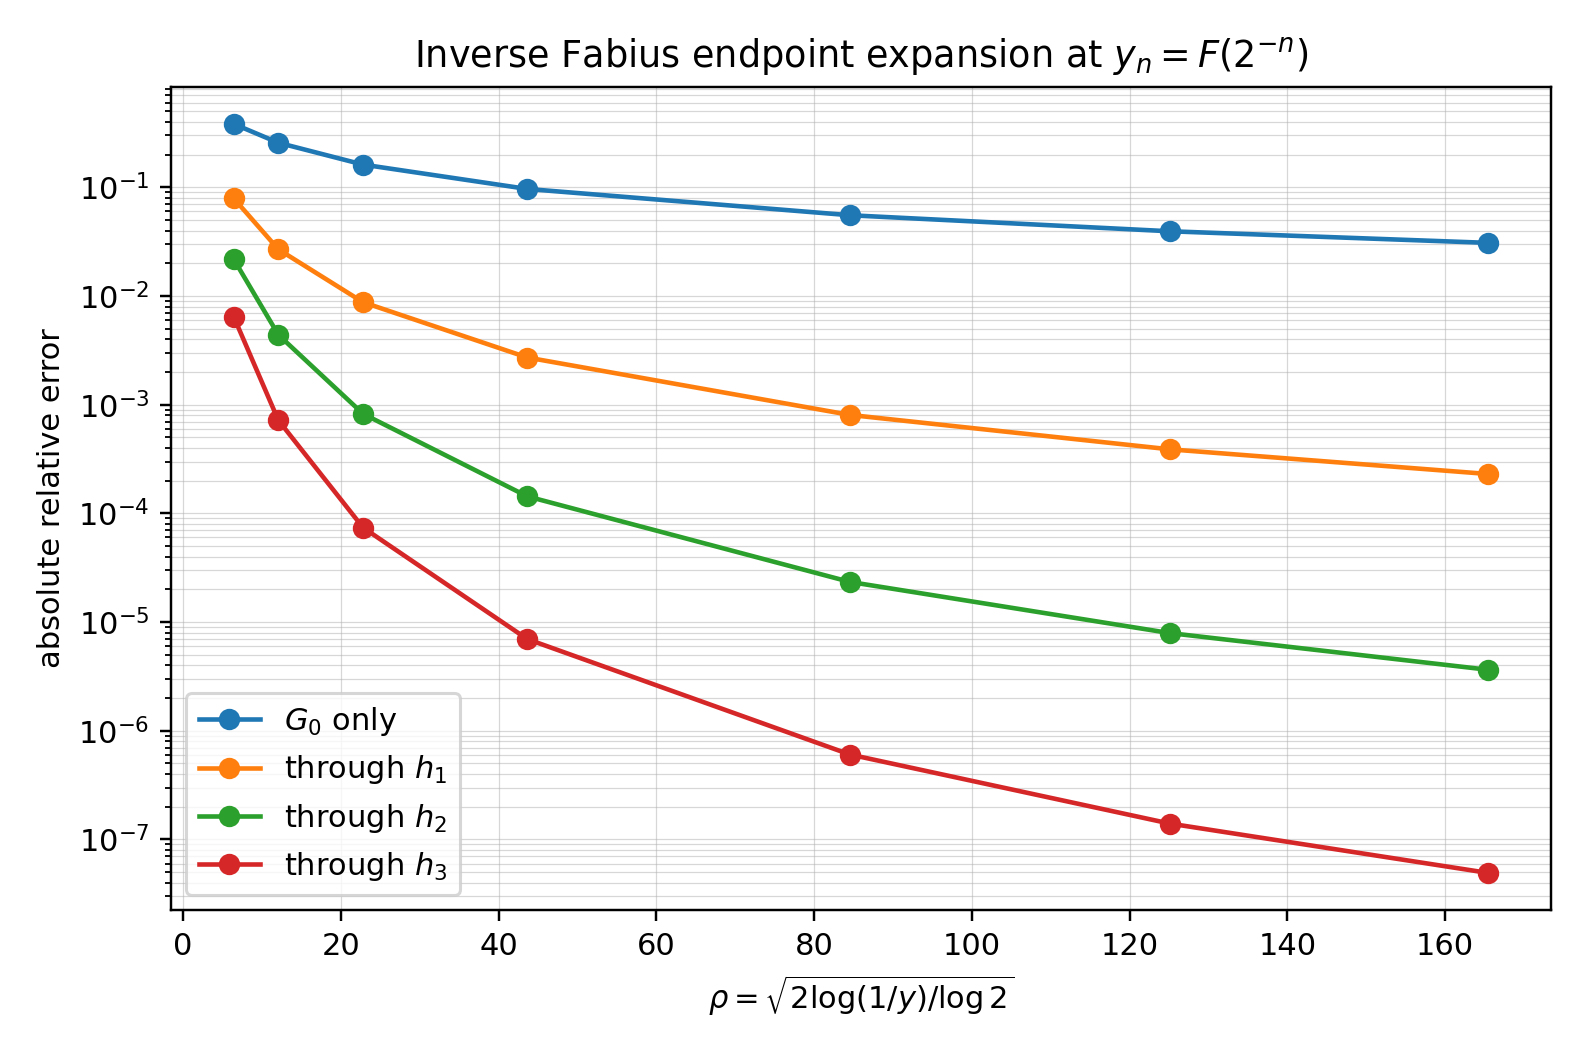
\includegraphics[width=0.82\textwidth]{results/endpoint_error_plot.png}
\caption{Absolute relative error on the exact dyadic quantiles.  Each additional logarithmic correction produces the expected strong reduction once $\rho$ is moderately large.}
\label{fig:error-plot}
\end{figure}

The new third correction improves the error by a factor of approximately
$11.1$ at $n=20$, $38.7$ at $n=80$, and $74.0$ at $n=160$ relative to the two-correction approximation.  The monotone improvement with depth is consistent with the fixed-order theorem; the finite-$n$ signs are not asserted to be universal.

\subsection{Reproducibility command}
From the package directory, run
\begin{lstlisting}[style=reportcode,language=bash]
python inverse_fabius_asymptotics.py --output-dir results \
    --precision 100 --modes 12 --depths 5 10 20 40 80 120 160
\end{lstlisting}
The script writes the exact-check log, constants, CSV table, and both PDF and PNG versions of \cref{fig:error-plot}.  It uses no network access.

\section{Equivalent forms and connections across the corpus}
\label{sec:connections}

\subsection{A literal expansion in the small argument}
The formulas can be stated without the auxiliary symbol $\rho$.  Put
\begin{equation}
 R(T)=\sqrt{\frac{2T}{L}},
 \qquad
 \Lambda(T)=\frac12\log\frac{2T}{L},
 \qquad
 \Theta(T)=R(T)+\beta.
 \label{eq:T-dictionary}
\end{equation}
Then the complete expansion is
\begin{align}
 G(y)={}&\frac{\sqrt T}{\e\sqrt L}
 \exp(-\sqrt{2LT})
 \notag\\
 &\times\exp\left\{
 \sum_{n=1}^{N}
 \left(\frac{L}{2T}\right)^{n/2}
 h_n\bigl(\Lambda(T),\Theta(T)\bigr)
 \right\}
 \notag\\
 &\times\left[1+
 \cO_N\left(
 \frac{(1+\log T)^N}{T^{(N+1)/2}}
 \right)\right],
 \qquad T=\log(1/y)\to\infty.
 \label{eq:literal-y-expansion}
\end{align}
Equivalently, the multiplicative normalization gives
\begin{align}
 G(y)={}&\frac{\sqrt T}{\e\sqrt L}\exp(-\sqrt{2LT})
 \left[1+\sum_{n=1}^{N}
 \left(\frac{L}{2T}\right)^{n/2}
 g_n\bigl(\Lambda(T),\Theta(T)\bigr)\right.
 \notag\\
 &\left.\hspace{8em}+
 \cO_N\left(\frac{(1+\log T)^{N+1}}{T^{(N+1)/2}}\right)\right].
 \label{eq:literal-g-expansion}
\end{align}
The phase $\Theta(T)$ is not an optional decoration: its periodic oscillation is of the same order as the nonoscillatory part of each coefficient.

\subsection{\texorpdfstring{Lambert--$W$ geometry}{Lambert W geometry}}
The forward endpoint is naturally parameterized by the exact identity
\begin{equation}
 x=\lambda e^{-L\lambda},
 \qquad
 \lambda=-\frac1L W_{-1}(-Lx).
 \label{eq:Lambert-geometry}
\end{equation}
A direct inversion in $x$ would repeatedly expand $W_{-1}$ and generate nested logarithms.  The present method instead performs the probabilistic/saddle inversion in $\lambda$ and invokes the Lambert identity only once, through \cref{eq:ratio-exact}.  This separation explains why the coefficient algebra is polynomial in $\ell=\log\rho$ rather than an uncontrolled nest of logarithms.

The constant shift $\beta=1/L+1/2$ has a geometric role: it completes the square in the dominant quadratic exponent.  The leading factor
\begin{equation}
 \Gzero=\rho e^{-L\rho-L\beta}
 \label{eq:G0-Lambert}
\end{equation}
is simply the Lambert map evaluated at the centered saddle phase $\rho+\beta$, with the small reversion $D$ removed.

\subsection{Bell and Bernoulli structures}
Two distinct Bell-polynomial mechanisms occur.
\begin{enumerate}
\item The forward saddle coefficients $A_j$ are differential polynomials assembled from exponential Bell polynomials in the local saddle jets.
\item The inverse multiplicative coefficients $g_n$ are complete Bell polynomials in the logarithmic coefficients $h_j$, as in \cref{eq:Bell-gn}.
\end{enumerate}
The diagonal Lagrange--B\"urmann formula links these mechanisms without flattening either one.  It can therefore be viewed as a ``Bell-of-Bell'' transform with an additional diagonal grading.

Bernoulli numbers and Bernoulli polynomials enter the forward analysis through Euler--Maclaurin corrections and the expansion of logarithmic factors.  On the inverse side, the elementary series
\begin{equation}
 \log(1+\beta z+zD)
 \label{eq:inverse-log-factor}
\end{equation}
is responsible for the rational terms $-\beta/2$, $-\beta^2/4$, and $\beta^3/3$ seen in \cref{eq:d2-known,eq:d3,eq:h3}.  At higher orders these elementary contributions can be organized with ordinary Bell polynomials or, after centering, Bernoulli-polynomial translation identities.

\subsection{Thue--Morse, q-binomial, and exact dyadic data}
The signed Thue--Morse sequence controls finite dyadic products and finite-difference cancellations throughout the corpus.  Gaussian q-binomial identities provide exact formulas for dyadic Fabius values and moment recurrences.  In the present report their most concrete role is verification: \cref{eq:dyadic-an,eq:dyadic-F} produce exact rational ordinates $y_n$ whose inverse is known exactly.

There is also a structural analogy.  The q-binomial side is graded by dyadic depth, while the inverse expansion is graded by the endpoint scale $z=1/\rho$.  In each case triangular recurrences coexist with closed coefficient extractions.  The diagonal formula \cref{eq:diagonal-dn} suggests searching for a direct q-series packaging of the inverse coefficients, rather than treating the dyadic exact values and continuous endpoint asymptotics as separate subjects.

\subsection{The Rvachev sinc product}
With the standard normalization, the compactly supported Rvachev function is the symmetric bell
\begin{equation}
 \operatorname{up}(x)=F(1-|x|),
 \qquad |x|\le1,
 \label{eq:up-F-relation}
\end{equation}
continued by zero outside its support.  Its Fourier transform is an infinite product of sinc factors at dyadic scales.  This spectral product explains the simultaneous appearance of dyadic self-similarity, very rapid smoothness, and special exact values.

The inverse endpoint asymptotics describe the geometry of extremely small level sets of the left flank of this bell.  Consequently, \cref{eq:phase-locked-expansion} may be read as an all-orders formula for the inward displacement from the support boundary at a prescribed tiny height.  The Gamma--zeta oscillation is a Mellin shadow of the same dyadic scale lattice that generates the sinc product.

\begin{statusbox}[Cross-corpus synthesis]
The chain of structures is
\[
 \begin{gathered}
 \text{dyadic sinc product}
 \longleftrightarrow \text{Thue--Morse/q-products}
 \longleftrightarrow \text{Mellin lattice and }\Psi,\\[0.25em]
 \text{saddle coefficients }A_j
 \longrightarrow \text{diagonal inverse coefficients }d_n,h_n,g_n.
 \end{gathered}
\]
The first line and the construction of $A_j$ are developed in the repository.  The final diagonal arrow is made closed and explicit in this report.
\end{statusbox}

\section{Conjectures and frontier directions}
\label{sec:conjectures}

The fixed-order expansion is rigorous.  Questions about order $N\to\infty$, optimal truncation, and complex continuation remain open and appear to contain the most interesting next layer.

\subsection{Large-order growth and resurgence}
The nearest boundary of the proved common analyticity strip is
\begin{equation}
 \sigma_* = \frac{\pi}{2L}.
 \label{eq:sigma-star}
\end{equation}
The inverse top-jet contribution to $h_n$ combines a derivative of order
$2n-2$ with a divisor $(n-1)!$.  Cauchy's estimate at distance $\sigma_*$ gives the heuristic scale
\begin{equation}
 \frac{(2n)!}{2^n n!L^{2n}}\sigma_*^{-2n}
 \asymp \frac{n!}{\sqrt{\pi n}}
 \left(\frac8{\pi^2}\right)^n.
 \label{eq:Gevrey-heuristic}
\end{equation}
This is factorial, but only Gevrey order one.

\begin{conjecture}[Gevrey-one inverse expansion]
\label{conj:Gevrey}
On every compact real phase set and for fixed bounded $\ell$, the coefficient families satisfy bounds of the form
\begin{equation}
 |h_n(\ell,\theta)|+|g_n(\ell,\theta)|
 \le C(\ell)A^n n!,
 \label{eq:Gevrey-bound}
\end{equation}
with the optimal exponential constant controlled by $8/\pi^2$ after the forward normalization is fixed.  The Borel transforms have their nearest singularities at locations generated by the complex phase boundaries and their dyadic translates.
\end{conjecture}

The value $8/\pi^2$ is a top-jet heuristic, not yet a proof of the exact large-order constant: other saddle diagrams may reinforce or partially cancel it.  A productive route is to combine the forward Bell recurrence with majorant series in a complex strip, then transport the resulting bounds through \cref{eq:diagonal-dn}.

\begin{conjecture}[Optimal truncation]
\label{conj:optimal-truncation}
For a fixed real phase, truncating near
\begin{equation}
 N_{\mathrm{opt}}\sim\frac{\pi^2}{8}\rho
 \label{eq:Nopt}
\end{equation}
produces an exponentially small remainder.  Its leading exponential and Stokes multiplier are governed by the nearest complex singularities of $\Psi$ together with the lower-Lambert branch geometry.
\end{conjecture}

\subsection{Persistence and geometry of oscillations}
\begin{conjecture}[Nonconstant phase at every order]
\label{conj:nonconstant}
For every $n\ge1$, each of $d_n(\ell,\theta)$, $h_n(\ell,\theta)$, and $g_n(\ell,\theta)$ has a nonconstant periodic component for generic $\ell$.  Equivalently, no finite truncation beyond the elementary leading factor becomes phase blind.
\end{conjecture}

The top-jet law makes this highly plausible, but a proof must exclude a special differential identity satisfied by $\Psi$ that cancels all nonzero Fourier modes at some order.  A certified proof could use the first Fourier mode, explicit convolution bounds for all nonlinear terms, and the enormous exponential gap between $|k|=1$ and $|k|\ge2$.

At first order the cluster set is an interval.  At higher order, after removal of logarithmic layers, one obtains images of the circle under vector-valued maps assembled from
$\Psi,\Psi',\ldots$.  Their self-intersections, curvature, and Fourier winding numbers form a new ``quantile cluster geometry.''

\begin{conjecture}[Generic embedded coefficient curves]
\label{conj:embedded-curves}
For a generic finite selection of renormalized inverse observables, the phase map into $\R^d$ is an immersed analytic closed curve; for sufficiently rich jet selections it is embedded.  The minimal embedding dimension is controlled by the first few nonzero Gamma--zeta modes.
\end{conjecture}

\subsection{Certified one-mode and few-mode asymptotics}
The first Fourier coefficient has magnitude about $10^{-6}$, while the decay exponent is $\pi^2/L\approx14.24$ per frequency.  This suggests a practical theorem: retain the mean and the first conjugate pair in every coefficient, propagate them through the diagonal algebra, and bound the discarded convolution tail by \cref{eq:fourier-truncation-bound}.  The output would be a short elementary trigonometric approximation with a rigorous error bar, useful for arbitrary-precision inversion without evaluating many special functions.

A stronger program is to precompute the Fourier-polynomial coefficient tables
\begin{equation}
 g_n(\ell,\theta)\approx
 \sum_{r=0}^{n}\sum_{|k|\le K}c_{n,r,k}\ell^r e^{2\pi\ii k\theta}
 \label{eq:coefficient-table}
\end{equation}
with interval-certified coefficients.  Combined with one Newton step on the exact functional equation, this should give a fast globally certified endpoint quantile algorithm.

\subsection{General dyadic and non-dyadic smoothing laws}
The mechanism is not restricted to the classical Fabius function.  Consider smoothing distributions whose Mellin transforms have a scale lattice generated by a base $b>1$, or compactly supported bells whose Fourier transforms are products
\begin{equation}
 \prod_{j\ge0}\operatorname{sinc}(c_jt)
 \label{eq:general-sinc-product}
\end{equation}
with geometric or eventually geometric $c_j$.  Their endpoint logarithms should again have a quadratic main phase, a log-periodic Mellin fluctuation, and differential-polynomial saddle corrections.

\begin{conjecture}[Universal diagonal inversion class]
\label{conj:universal-class}
Whenever a distribution has a forward exact-phase expansion of the form
\begin{equation}
 -a\lambda^2+b\lambda-c\log\lambda+C+P(\lambda)
 +\sum_{j\ge1}A_j(\lambda)\lambda^{-j},
 \label{eq:universal-forward-form}
\end{equation}
with periodic analytic $P,A_j$, its inverse admits a diagonal Lagrange--B\"urmann expansion with polynomial logarithms, phase-locked subsequences, a newest-jet transfer law, and a Bell-polynomial multiplicative conversion.  The universal highest logarithms depend only on $a$ and $c$.
\end{conjecture}

Proving this abstract theorem would clarify which features are specifically dyadic and which belong to a wider universality class of log-periodically perturbed Gaussian tails.

\subsection{Uniform high derivatives and complex quantiles}
The recurrence \cref{eq:Q-recurrence} solves the fixed-$m$ derivative problem.  It does not control the double limit $m,\rho\to\infty$.  A two-parameter saddle analysis could identify the transition scale at which the harmonic correction $\mathsf H_{m-1}/\rho$ ceases to be small and endpoint sign alternation changes character.

Complex continuation is equally promising.  The exact phase uses $W_{-1}$ on the real axis, but complex inverse branches interact with the periodic strip singularities.  Locating the nearest complex critical values of $F$ would determine the analytic continuation radius of $G$ around tiny positive $y$ and should connect directly to the Borel singularities in \cref{conj:Gevrey,conj:optimal-truncation}.

\subsection{Formal verification}
The coefficient theorem is well suited to computer-assisted proof.  Its core is formal power-series algebra over a differential coefficient ring.  A Lean development could proceed in four modules:
\begin{enumerate}
\item formal Lagrange--B\"urmann inversion with a parameter $z$;
\item the diagonal extraction theorem \cref{eq:diagonal-dn};
\item polynomial-logarithmic degree and top-jet filtrations;
\item analytic transfer from formal cancellation to the fixed-order remainder using \cref{eq:large-implicit-derivative}.
\end{enumerate}
The accompanying SymPy checks provide test vectors but are not substitutes for such a proof.

\section{Conclusion}
\label{sec:conclusion}

The inverse Fabius endpoint is governed by three coupled scales:
\begin{equation}
 \text{Gaussian magnitude }T,
 \qquad
 \text{slow logarithm }\ell=\tfrac12\log(2T/L),
 \qquad
 \text{dyadic phase }\theta=\sqrt{2T/L}+\beta.
\end{equation}
The repository had already identified these scales, proved the all-orders forward expansion, and constructed a recursive inverse continuation.  The central advance of this report is to close the coefficient problem: every inverse coefficient is now a finite diagonal Lagrange--B\"urmann extraction, with direct companion formulas for both logarithmic and multiplicative normalizations.

This closed calculus reveals structural laws that are difficult to see recursively.  The multiplicative highest logarithm is universal, the newest periodic derivative transfers from $A_{n-1}$ with a simple coefficient, every Fourier mode is a finite Gamma--zeta convolution, and every fixed ordinary derivative follows from one differential recurrence.  The explicit third correction is already numerically effective on exact dyadic quantiles.

The likely next frontier is not another isolated low-order term.  It is the large-order theory: Gevrey bounds, optimal truncation, Borel singularities, and a transseries that resolves the exponentially small remainder.  The diagonal formula provides a concrete algebraic foundation for that program.

\appendix

\section{Coefficient-extraction proof details}
\label{app:proof-details}

\subsection{Why the diagonal formula is finite}
For $d_n$, the summand with index $k$ in \cref{eq:diagonal-dn} asks for
$z^{n-k}w^{k-1}$.  Hence:
\begin{itemize}
\item no power $z^r$ of $\Phi$ with $r>n-k$ contributes;
\item no Taylor jet in $w$ above order $k-1$ contributes;
\item an $A_j$ term can occur only when $j\le n-k$.
\end{itemize}
Therefore $A_{n-1}$ appears only in the $k=1$ summand, which is also the key observation in the inverse top-jet proof.

\subsection{A partition form}
Expand
\begin{equation}
 \Phi(z,w)=\sum_{r,s\ge0}\phi_{r,s}z^rw^s.
 \label{eq:Phi-bivariate}
\end{equation}
Then \cref{eq:diagonal-dn} becomes the explicit finite composition sum
\begin{equation}
 d_n=\sum_{k=1}^{n}\frac1k
 \sum_{\substack{r_1+\cdots+r_k=n-k\\
 s_1+\cdots+s_k=k-1}}
 \prod_{j=1}^{k}\phi_{r_j,s_j}.
 \label{eq:dn-partition}
\end{equation}
This is a general coefficient formula with no implicit lower-order $d_j$.  Grouping equal pairs $(r,s)$ rewrites it as a multivariate ordinary Bell polynomial.  Formula \cref{eq:dn-partition} is often preferable for proof, while \cref{eq:diagonal-dn} is preferable for implementation.

\subsection{Formal-to-asymptotic transfer}
Let
\begin{equation}
 \mathscr F_y(w)=\frac Lzw+\mathcal R_N(z,w)+E_N(z,w),
 \label{eq:Fy}
\end{equation}
where $\mathcal R_N$ contains the retained $A_1,\ldots,A_{N-1}$ and
$E_N=\cO_N(z^N)$.  Formal cancellation gives
\begin{equation}
 \mathscr F_y(D^{[N]})=
 \cO_N((1+\ell)^Nz^N).
\end{equation}
The exact $D$ satisfies $\mathscr F_y(D)=0$.  For small enough $z$,
\begin{equation}
 \inf_w|\partial_w\mathscr F_y(w)|\ge\frac{L}{2z}
 \label{eq:implicit-lower-bound}
\end{equation}
throughout the relevant $\cO(\ell z)$ neighborhood.  Hence
\begin{equation}
 |D-D^{[N]}|\le \frac{2z}{L}
 |\mathscr F_y(D^{[N]})|
 =\cO_N((1+\ell)^Nz^{N+1}).
 \label{eq:D-error-transfer}
\end{equation}
This elementary gain-of-one-power argument is why a forward expansion through $A_{N-1}$ suffices for an inverse phase expansion through $d_N$.

\section{Corpus audit ledger}
\label{app:audit}

The audit covered every LaTeX source exposed under the requested directory and its subdirectories at the time of access.  The tree was actively consolidated on 28 August 2026, so file counts in older internal manifests and the living tree do not coincide.  To keep the provenance useful after renames, the ledger below records stable source families and recognizable file stems rather than asserting a permanently frozen count.

\begin{longtable}{@{}>{\raggedright\arraybackslash}p{0.34\textwidth}p{0.58\textwidth}@{}}
\caption{Stable source families used in the corpus audit.}\label{tab:audit-ledger}\\
\toprule
Family or file stem & Material checked for duplication and used as context \\
\midrule
\endfirsthead
\toprule
Family or file stem & Material checked for duplication and used as context \\
\midrule
\endhead
\path{Fabius_Function_and_Rvachev_Up} & Main normalization, functional equations, exact values, moments, Fourier/product identities, endpoint discussion. \\
\path{FabiusFunction_Mathematical_Glossary} & Notation dictionary, theorem crosswalk, constants, special-function conventions. \\
\path{Non_Elementarity} & Differential-algebraic context and restrictions on elementary closed forms. \\
\path{fabius_lean_walkthrough} & Formalized definitions and theorem correspondence. \\
\path{non-formalized-research-frontiers} & Exact-phase saddle expansion, coefficient recurrences, Bell-polynomial formulas, top-jet results, open problems. \\
\path{Inverse_and_Sampling_Frontiers} & Leading inverse equivalent, first two corrections, cluster interval, elasticity, all-order triangular recursion, sampling questions. \\
\path{Thue_Morse_Atlas_and_Frontiers} and earlier Thue--Morse drafts & Signed/unsigned sequence formulas, finite products, exact dyadic identities, spectral and q-series links. \\
\path{Exponents_and_q_Series_Frontiers} & Gaussian q-binomial formulas, exponent arithmetic, finite-depth recurrences. \\
\path{Spectra_and_Arithmetic_Frontiers} & Fourier/Mellin spectra, arithmetic values, Dirichlet and Gamma--zeta structures. \\
\path{Integration_and_Transform_Frontiers}; \path{Fabius_Integral_Transforms_Report} & Mellin, Laplace, Fourier, resolvent, and integral-transform representations. \\
\path{Representation_Frontiers}; \path{Representation_Second_Wave} & Shift/scale systems, polynomial reproduction, multiresolution, moment representations. \\
\path{Frontier_Compilations} & Consolidated reports and cross-topic theorem indexes. \\
Fourier-decay and sinc-product sources & Partial and infinite sinc products, dyadic spectral decay, Rvachev approximants, numerical Fourier analysis. \\
Archived small-argument and asymptotic notes & Earlier leading and subleading endpoint formulas, Lambert--$W$ approximations, historical normalizations. \\
Embedded paper transcriptions & Classical Fabius/Rvachev sources, arithmetic evaluations, smooth compactly supported functions, computational methods. \\
Interpolation, summation, integration, and representation reports & Screened for inverse expansions, coefficient formulas, and derivative laws so that adjacent new work was not inadvertently repeated. \\
\bottomrule
\end{longtable}

The immediate novelty comparison was made against the living inverse-focused report, not merely against older archived notes.  In particular, the first two corrections and the triangular all-orders engine are explicitly credited as prior repository results throughout this report.

\section{Reproducibility files and implementation notes}
\label{app:reproducibility}

The archive accompanying this report contains:
\begin{center}
\begin{tabularx}{0.94\textwidth}{@{}p{0.40\textwidth}X@{}}
\toprule
File & Purpose \\
\midrule
\path{inverse_fabius_all_orders.tex} & Complete report source. \\
\path{inverse_fabius_all_orders.pdf} & Rendered report. \\
\path{inverse_fabius_asymptotics.py} & Exact dyadic recurrence, Gamma--zeta evaluation, diagonal/triangular symbolic checks, tables, plot. \\
\path{results/endpoint_errors.csv} & Full-precision numerical table underlying \cref{tab:dyadic-errors}. \\
\path{results/symbolic_checks.txt} & Exact SymPy identity log. \\
\path{results/constants.txt} & Constants and leading Fourier mode at 100 digits. \\
\path{results/endpoint_error_plot.pdf} & Vector version of the error plot. \\
\path{results/endpoint_error_plot.png} & Raster version included in this PDF. \\
\bottomrule
\end{tabularx}
\end{center}

The exact rational recurrence is deliberately separated from the asymptotic evaluator.  This prevents numerical evaluation of $F$ or numerical root finding from masking an error in the inverse expansion.  The symbolic checker likewise treats the forward jets as independent variables; it therefore checks algebraic reversion rather than only one numerical realization of $\Psi$.

\section{Selected notation}
\label{app:notation}

\begin{longtable}{@{}p{0.23\textwidth}p{0.67\textwidth}@{}}
\caption{Notation used throughout the report.}\label{tab:notation}\\
\toprule
Symbol & Meaning \\
\midrule
\endfirsthead
\toprule
Symbol & Meaning \\
\midrule
\endhead
$F$, $G$ & Fabius function and its inverse. \\
$L$ & $\log2$. \\
$B$ & $1+L/2$. \\
$\beta$ & $B/L=1/L+1/2$. \\
$T$ & $\log(1/y)$. \\
$\rho$ & $\sqrt{2T/L}$. \\
$z$ & $1/\rho$. \\
$\ell$ & $\log\rho$. \\
$\theta$ & $\rho+\beta$, interpreted modulo one inside periodic functions. \\
$\lambda(x)$ & $-W_{-1}(-Lx)/L$, so $x=\lambda e^{-L\lambda}$. \\
$\Psi$ & Mean-zero one-periodic Gamma--zeta endpoint fluctuation. \\
$A_j$ & Periodic forward saddle coefficients. \\
$D$ & Phase displacement $\lambda(G(y))-\rho-\beta$. \\
$d_n$ & Coefficients of $D=\sum d_nz^n$. \\
$h_n$ & Coefficients of $\log(G/G_0)=\sum h_nz^n$. \\
$g_n$ & Coefficients of $G/G_0=1+\sum g_nz^n$. \\
$\Phi$ & Fixed-point kernel in $D=z\Phi(z,D)$. \\
$\mathcal E$ & Endpoint elasticity $yG'/G$. \\
$Q_m$ & Dimensionless derivative ratio $y^mG^{(m)}/G$. \\
\bottomrule
\end{longtable}

\begin{thebibliography}{99}

\bibitem{Fabius1966}
J.~Fabius,
\newblock A probabilistic example of a nowhere analytic $C^\infty$ function,
\newblock \emph{Zeitschrift f\"ur Wahrscheinlichkeitstheorie und Verwandte Gebiete} \textbf{5} (1966), 173--174.

\bibitem{Rvachev1990}
V.~L. Rvachev,
\newblock Compactly supported solutions of functional-differential equations and their applications,
\newblock \emph{Russian Mathematical Surveys} \textbf{45} (1990), no.~1, 87--120.

\bibitem{AlloucheShallit}
J.-P. Allouche and J.~Shallit,
\newblock \emph{Automatic Sequences: Theory, Applications, Generalizations},
\newblock Cambridge University Press, 2003.

\bibitem{Corless1996}
R.~M. Corless, G.~H. Gonnet, D.~E.~G. Hare, D.~J. Jeffrey, and D.~E. Knuth,
\newblock On the Lambert $W$ function,
\newblock \emph{Advances in Computational Mathematics} \textbf{5} (1996), 329--359.

\bibitem{Comtet}
L.~Comtet,
\newblock \emph{Advanced Combinatorics: The Art of Finite and Infinite Expansions},
\newblock D.~Reidel, 1974.

\bibitem{FlajoletSedgewick}
P.~Flajolet and R.~Sedgewick,
\newblock \emph{Analytic Combinatorics},
\newblock Cambridge University Press, 2009.

\bibitem{Olver}
F.~W.~J. Olver,
\newblock \emph{Asymptotics and Special Functions},
\newblock A K Peters, 1997 reprint.

\bibitem{DLMF}
NIST Digital Library of Mathematical Functions,
\newblock Chapters on the Gamma function, Riemann zeta function, asymptotic approximations, and Lambert $W$,
\newblock \url{https://dlmf.nist.gov/}.

\bibitem{Repository}
V.~Reshetnikov,
\newblock \emph{ProveIt: Analysis/FabiusFunction/docs}, living LaTeX research corpus,
\newblock \url{https://github.com/VladimirReshetnikov/ProveIt/tree/main/Analysis/FabiusFunction/docs}, accessed 28 August 2026.

\bibitem{RepoPrimary}
V.~Reshetnikov,
\newblock \emph{Fabius Function and Rvachev Up: primary exposition and mathematical glossary},
\newblock in \cite{Repository}.

\bibitem{RepoFrontier}
V.~Reshetnikov,
\newblock \emph{Non-formalized research frontiers for the Fabius and Rvachev functions},
\newblock in \cite{Repository}.

\bibitem{RepoInverse}
V.~Reshetnikov,
\newblock \emph{Inverse and Sampling Frontiers},
\newblock in \cite{Repository}, living draft inspected 28 August 2026.

\bibitem{RepoManifest}
V.~Reshetnikov,
\newblock Draft manifest and thematic consolidation notes,
\newblock in \cite{Repository}, 28 August 2026.

\end{thebibliography}

\end{document}
